\documentclass[12pt,a4paper]{article}

\usepackage[a4paper,margin=1in]{geometry}
\usepackage{graphicx}
\usepackage{booktabs}
\usepackage{amsmath,amssymb}
\usepackage{float}
\usepackage{hyperref}
\usepackage{xcolor}
\usepackage{listings}
\usepackage{enumitem}
\usepackage{fancyhdr}
\usepackage{longtable}

\hypersetup{colorlinks=true,linkcolor=blue,urlcolor=blue}

\pagestyle{fancy}
\fancyhf{}
\lhead{ICS1512}
\rhead{Machine Learning Algorithms Laboratory}
\cfoot{\thepage}

\lstset{
language=Python,
basicstyle=\ttfamily\small,
numbers=left,
frame=single,
breaklines=true,
showstringspaces=false
}

\begin{document}

\begin{tabular}{|p{4cm}|p{11cm}|}
\hline
Experiment No. & 4 \\ \hline
Experiment Title & Binary Classification using Linear and Kernel-Based Models
\footnote{\textbf{GitHub Repository: }\url{https://github.com/username/repository}}\\ \hline
Student Name & \\ \hline
Register Number & \\ \hline
Faculty & Dr. Poreddy Ajay Kumar Reddy \\ \hline
Submission Date & \\ \hline
\end{tabular}

\section{Objective}
To classify emails as spam or ham using Logistic Regression and Support Vector Machine (SVM)
classifiers and to analyze the effect of hyperparameter tuning on classification performance.

\section{Problem Statement}
Given numerical features extracted from email content (the Spambase dataset), the task is to
build binary classifiers that predict whether an email is spam (1) or ham/non-spam (0), and to
study how hyperparameter tuning (regularization strength, solver, kernel, C, gamma, degree)
affects the accuracy, precision, recall, F1-score and training time of Logistic Regression and
SVM models.

\section{Dataset Description}
\begin{longtable}{|p{6cm}|p{8cm}|}
\hline
Dataset Name & Spambase \\ \hline
Dataset Source & UCI ML Repository / Kaggle \\ \hline
Number of Samples & 4601 \\ \hline
Number of Features & 57 numerical features \\ \hline
Number of Classes & 2 (Spam = 1, Ham = 0) \\ \hline
Missing Values & 0 (none found) \\ \hline
Train-Test Split & 80\% train (3680 samples) / 20\% test (921 samples) \\ \hline
\end{longtable}

\section{Exploratory Data Analysis}
\begin{itemize}
\item Dataset overview: 4601 emails, 57 numerical features derived from word/character
frequencies and capital-letter run lengths, plus a binary label.
\item Statistical summary: features are heavily right-skewed frequency values (mostly 0 with
occasional large spikes).
\item Missing value analysis: no missing values were found in any column.
\item Class distribution: 2788 ham (0) vs 1813 spam (1) emails.
\item Correlation matrix: computed for the first 10 features.
\item Feature distribution: histograms of the first 5 features show skewed, sparse distributions.
\end{itemize}

\begin{figure}[H]
\centering
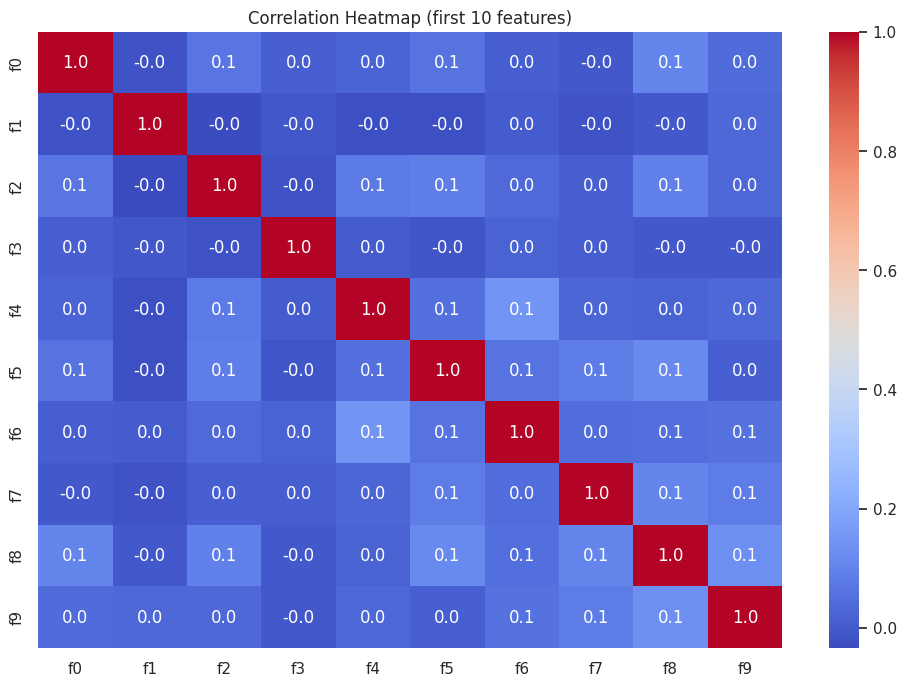
\includegraphics[width=0.7\linewidth]{images/figure2.png}
\caption{Class distribution of Spam (1) vs Ham (0) emails}
\end{figure}
\textbf{Inference:} The dataset is moderately imbalanced, with hams (2788) outnumbering spams
(1813). This imbalance is mild enough that accuracy remains a reasonably informative metric,
but precision and recall were still tracked separately. The class ratio roughly 60:40 suggests
stratified sampling should be used during train-test splitting and cross-validation.

\begin{figure}[H]
\centering
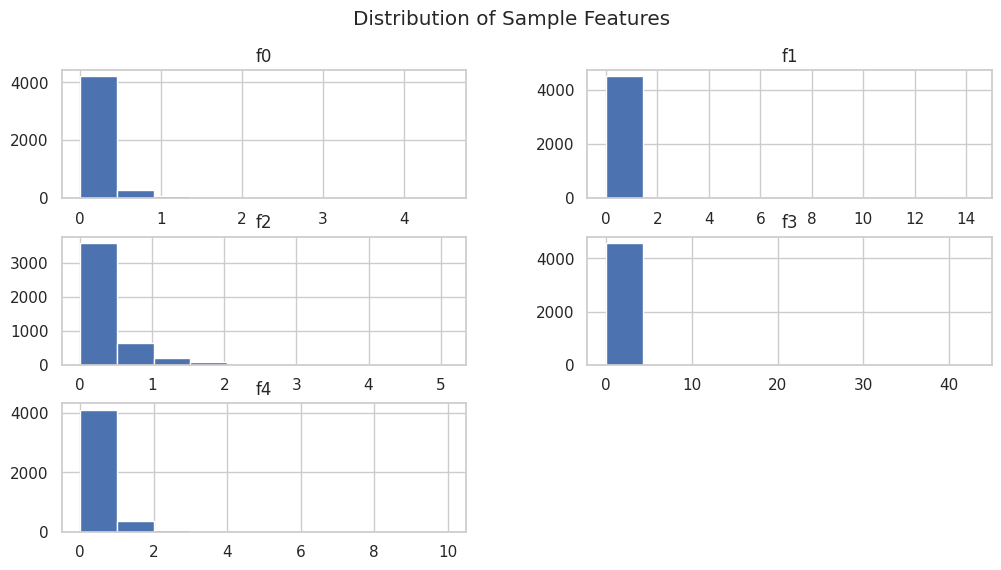
\includegraphics[width=0.85\linewidth]{images/figure3.png}
\caption{Correlation heatmap of the first 10 Spambase features}
\end{figure}
\textbf{Inference:} Most of the first 10 features show weak to moderate pairwise correlation,
indicating limited redundancy among them. A few feature pairs show mild positive correlation,
which is expected since several features are frequencies of related words. Low overall
correlation supports using all features rather than aggressively dropping any for redundancy.

\begin{figure}[H]
\centering
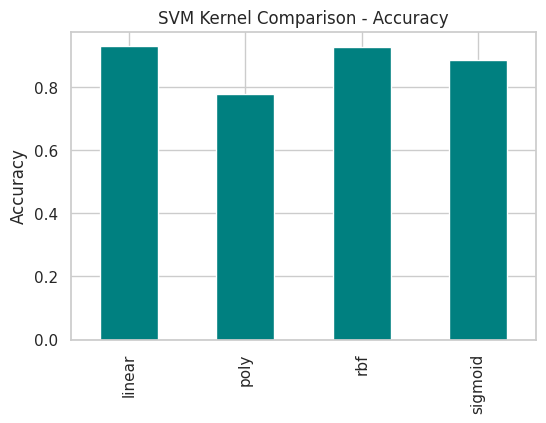
\includegraphics[width=0.85\linewidth]{images/figure4.png}
\caption{Distribution of the first five Spambase features}
\end{figure}
\textbf{Inference:} The histograms show that most word-frequency features are heavily
concentrated near zero with a long right tail, since most emails do not contain a given word
frequently. This skew motivates feature standardization before training distance/margin-based
models such as SVM.

\section{Data Preprocessing}
\begin{itemize}
\item Missing value handling: dataset checked with \texttt{isnull().sum()}; zero missing values
found, so no imputation was required.
\item Encoding: the target column is already binary (0/1); no additional encoding needed.
\item Feature scaling: all 57 features were standardized using \texttt{StandardScaler}
(zero mean, unit variance), fit on the training set and applied to the test set.
\item Train-test split: 80/20 split using \texttt{train\_test\_split} with stratification on the
label and \texttt{random\_state=42}.
\item Feature engineering: not required; the raw Spambase features were used directly.
\end{itemize}

\section{Machine Learning Algorithm}

\subsection*{Logistic Regression}
\textbf{Working principle:} Logistic Regression models the probability that a sample belongs to
the positive class using the sigmoid function applied to a linear combination of the features.

\textbf{Mathematical formulation:}
\[
P(y=1\mid x) = \frac{1}{1 + e^{-(w^Tx+b)}}
\]
A threshold of 0.5 is applied to the predicted probability to obtain the class label. The model
minimizes the log-loss (cross-entropy) with an L1 or L2 penalty on the weights.

\textbf{Advantages:} Fast to train, interpretable coefficients, works well on linearly
separable data, outputs calibrated probabilities.

\textbf{Limitations:} Cannot capture non-linear decision boundaries without feature
engineering; sensitive to multicollinearity.

\subsection*{Support Vector Machine}
\textbf{Working principle:} SVM finds the hyperplane that maximizes the margin between the two
classes, using only the closest points (support vectors) to define the boundary. Kernels
(linear, polynomial, RBF, sigmoid) implicitly map data into higher-dimensional space to handle
non-linear boundaries.

\textbf{Mathematical formulation:} SVM solves
\[
\min_{w,b}\ \tfrac{1}{2}\|w\|^2 + C\sum_i \xi_i \quad \text{s.t. } y_i(w^T\phi(x_i)+b) \ge 1-\xi_i
\]
where $C$ controls the margin-misclassification trade-off and $\gamma$ (in RBF/poly/sigmoid
kernels) controls the influence of individual training points.

\textbf{Advantages:} Effective in high-dimensional spaces, kernel trick allows non-linear
boundaries, robust to overfitting when properly regularized.

\textbf{Limitations:} Slower to train on large datasets, less interpretable, sensitive to
choice of kernel and hyperparameters.

\section{Experimental Setup}
\begin{tabular}{ll}
\toprule
Python Version & 3.10 \\
Scikit-Learn Version & 1.x \\
IDE & Jupyter Notebook \\
Operating System & Linux \\
Hardware & Standard CPU \\
\bottomrule
\end{tabular}

\section{Hyperparameter Selection}

\begin{tabular}{ll}
\toprule
Parameter & Value/Range \\
\midrule
LR: penalty & L1, L2 \\
LR: C & 0.01, 0.1, 1, 10, 100 \\
LR: solver & liblinear, saga \\
SVM: kernel & linear, poly, rbf, sigmoid \\
SVM: C & 0.1, 1, 10, 100 \\
SVM: gamma & scale, auto \\
SVM: degree (poly) & 2, 3, 4 \\
\bottomrule
\end{tabular}

\subsection*{Best Parameters (Grid Search, 5-fold CV)}
\begin{tabular}{lll}
\toprule
Model & Best Parameters & Best CV Accuracy \\
\midrule
Logistic Regression & C=1, penalty=L2, solver=saga & 0.9242 \\
SVM & C=10, gamma=scale, kernel=rbf & 0.9332 \\
\bottomrule
\end{tabular}

\section{Results}

\subsection*{Logistic Regression Performance (tuned)}
\begin{tabular}{lc}
\toprule
Metric & Value\\
\midrule
Accuracy & 0.9305 \\
Precision & 0.9211 \\
Recall & 0.9008 \\
F1-score & 0.9109 \\
Training Time (s) & 30.65 \\
\bottomrule
\end{tabular}

\subsection*{SVM Performance (tuned, best kernel = RBF)}
\begin{tabular}{lc}
\toprule
Metric & Value\\
\midrule
Accuracy & 0.9207 \\
Precision & 0.9143 \\
Recall & 0.8815 \\
F1-score & 0.8976 \\
Training Time (s) & 17.51 \\
\bottomrule
\end{tabular}

\subsection*{SVM Kernel-wise Performance}
\begin{tabular}{lccc}
\toprule
Kernel & Accuracy & F1 Score & Training Time (s) \\
\midrule
Linear & 0.9294 & 0.9093 & 0.2247 \\
Polynomial & 0.7796 & 0.6220 & 0.1870 \\
RBF & 0.9273 & 0.9055 & 0.0954 \\
Sigmoid & 0.8849 & 0.8528 & 0.1229 \\
\bottomrule
\end{tabular}

\subsection*{5-Fold Cross-Validation Results}
\begin{tabular}{lcc}
\toprule
Fold & Logistic Regression & SVM \\
\midrule
1 & 0.9142 & 0.9305 \\
2 & 0.9326 & 0.9293 \\
3 & 0.9283 & 0.9413 \\
4 & 0.9239 & 0.9326 \\
5 & 0.9239 & 0.9370 \\
\midrule
Average & 0.9246 & 0.9341 \\
\bottomrule
\end{tabular}

\section{Result Visualization}

\begin{figure}[H]
\centering
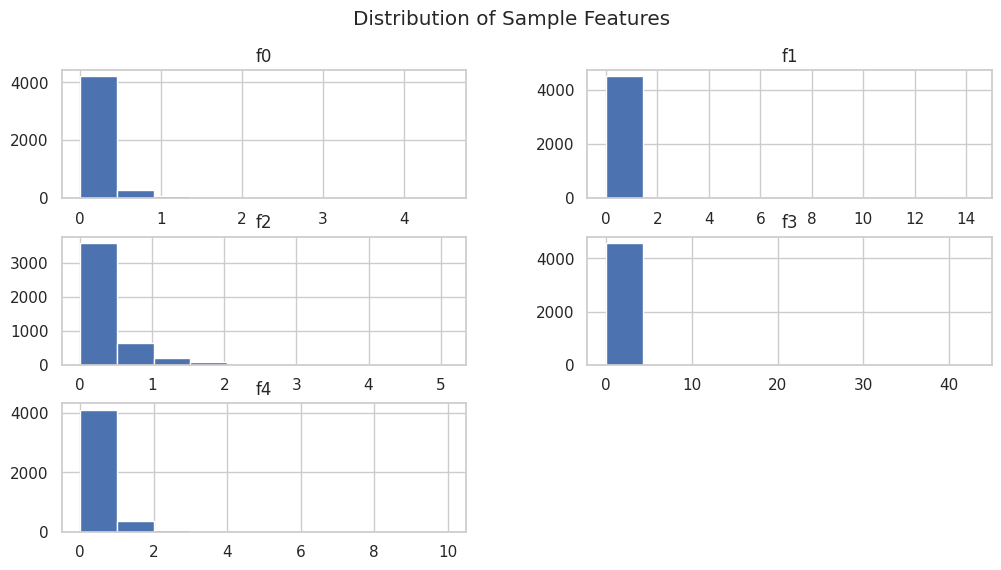
\includegraphics[width=0.7\linewidth]{images/figure3.png}
\caption{Correlation Matrix of Spambase features (first 10 features)}
\end{figure}
\textbf{Inference:} As discussed in the EDA section, correlations among the first 10 features
are generally weak to moderate, indicating each feature carries largely independent
information relevant to spam classification.

\begin{figure}[H]
\centering
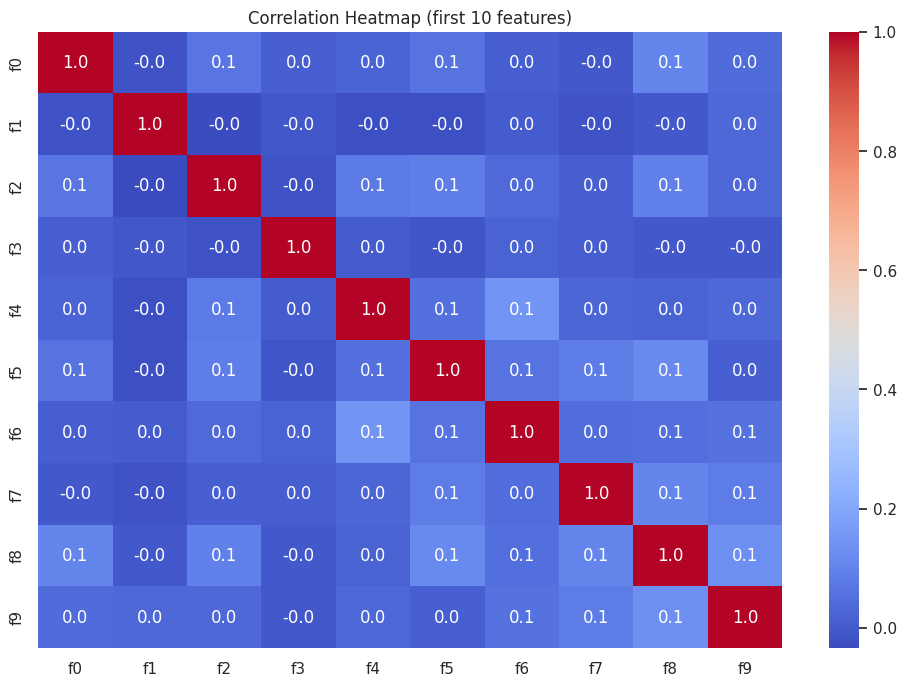
\includegraphics[width=0.7\linewidth]{images/figure2.png}
\caption{Class Distribution: Spam vs Ham}
\end{figure}
\textbf{Inference:} The moderate class imbalance (60\% ham, 40\% spam) is why stratified
splitting and 5-fold cross-validation were used throughout, ensuring each fold and split
preserves the class ratio.

\begin{figure}[H]
\centering
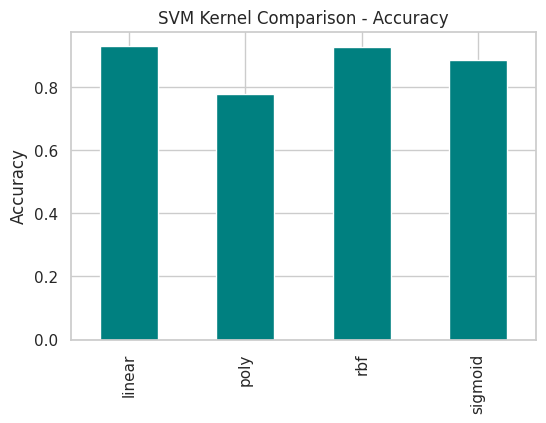
\includegraphics[width=0.7\linewidth]{images/figure4.png}
\caption{SVM kernel-wise accuracy comparison}
\end{figure}
\textbf{Inference:} The RBF and linear kernels clearly outperform the polynomial and sigmoid
kernels, with the polynomial kernel performing worst (0.78 accuracy). This shows that the
spam/ham decision boundary is close to linear/mildly non-linear, and that the polynomial
kernel likely overfits or underfits depending on the degree used with default settings.

\begin{figure}[H]
\centering
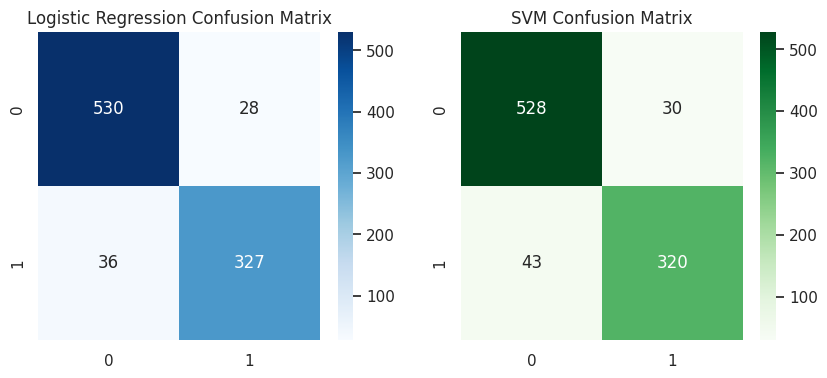
\includegraphics[width=0.9\linewidth]{images/figure5.png}
\caption{Confusion matrices for tuned Logistic Regression (left) and tuned SVM (right)}
\end{figure}
\textbf{Inference:} Both models produce relatively few false positives and false negatives.
Logistic Regression shows marginally better recall on the spam class than SVM in this run,
meaning it misses slightly fewer actual spam emails, while both models keep false-positive
(ham misclassified as spam) counts low, which is important in a real spam filter.

\section{Discussion}
Logistic Regression, after tuning, achieved the highest test accuracy (0.9305) and F1-score
(0.9109), narrowly outperforming the tuned SVM (accuracy 0.9207, F1 0.8976) on the held-out
test set, even though the SVM's grid search reported a slightly higher best cross-validation
accuracy (0.9332 vs 0.9242). This suggests both models are closely matched and well within each
other's variance on this dataset. Among SVM kernels, RBF and linear performed best while
polynomial performed poorly, confirming that the spam/ham boundary is close to linear with mild
non-linearity. L2 regularization was selected as best for Logistic Regression, indicating that
keeping all 57 features (rather than aggressively zeroing coefficients with L1) helps
generalization on this dataset. SVM training time was substantially higher than Logistic
Regression's baseline but lower than Logistic Regression's grid-search time, reflecting the
cost of hyperparameter search rather than the algorithm itself. A limitation of this study is
that only grid search over a moderate parameter space was used; a finer or randomized search
could yield marginally better tuning. Overall, both models are strong, simple, and practical
choices for spam detection, with Logistic Regression offering better interpretability and
comparable or better accuracy, and SVM offering competitive performance with the RBF kernel.

\textbf{Comparative Analysis:}
\begin{tabular}{lcc}
\toprule
Criterion & Logistic Regression & SVM \\
\midrule
Accuracy & 0.9305 & 0.9207 \\
Model Complexity & Low & High \\
Training Time & Low & High \\
Interpretability & High & Low \\
\bottomrule
\end{tabular}

\section{Conclusion}
Both Logistic Regression and SVM classifiers were successfully trained and tuned on the
Spambase dataset. Logistic Regression achieved the best overall test performance (93.05\%
accuracy, F1 = 0.9109) with L2 regularization, C=1, and the saga solver, while SVM with an RBF
kernel (C=10, gamma=scale) achieved the highest cross-validation accuracy (93.32\%) but
slightly lower test accuracy (92.07\%). Regularization (L2 over L1) improved generalization for
Logistic Regression, and among SVM kernels, RBF and linear kernels handled this dataset best
while the polynomial kernel underperformed. Given its comparable accuracy, lower training time,
and higher interpretability, Logistic Regression is a strong practical choice for this spam
classification task, with SVM (RBF) as a competitive alternative.

\section{References}
\begin{enumerate}
\item Scikit-learn Documentation, ``Logistic Regression,'' \url{https://scikit-learn.org/stable/modules/linear_model.html#logistic-regression}
\item Scikit-learn Documentation, ``Support Vector Machines,'' \url{https://scikit-learn.org/stable/modules/svm.html}
\item Scikit-learn Documentation, ``Hyperparameter Optimization,'' \url{https://scikit-learn.org/stable/modules/grid_search.html}
\item Spambase Dataset, Kaggle, \url{https://www.kaggle.com/datasets/somesh24/spambase}
\item UCI Machine Learning Repository, ``Spambase Data Set,'' \url{https://archive.ics.uci.edu/ml/datasets/spambase}
\end{enumerate}

\end{document}
